\documentclass[a4paper, 10pt]{article}
\usepackage{style}

% Début du document
\begin{document}
	\debut{2}{Projet PPC}{Olivier bailleux}
		\section{Principe}
            L'objectif est de réaliser une pré-génération, ce développement s'est découpé en deux phases, un développement de découverte et mise en place des fonctionnalités, puis une refonte du code pour optimiser l'algorithme.

            \subsection{Phase 1 - Mise en place des fonctionnalités}
                Dans un premier temps, implémentation d'un tirage au hasard \verb?k? fois en vérifiant simplement si la case n'était pas déjà utilisée. Suite à cela, ajout de la vérification des diagonales.

                Afin d'éviter que l'algorithme tourne indéfiniment, ajout d'une limite du nombre de tentative avant que le générateur ne s'arrête.

                \begin{description}
                    \item Répétition jusqu'à ce que \verb?k? soit atteint:
                    \begin{description}
                        \item Tirage au sort d'un \verb?X? et d'un \verb?Y?.
                        \item Vérification des diagonales.
                        \item Si pas de problème lors de la vérification des diagonales:
                        \begin{description}
                            \item Enregistrement de \verb?X? et \verb?Y? dans \verb?init?.
                            \item Remise à zéro du nombre de tentatives.
                        \end{description}
                        \item Sinon:
                        \begin{description}
                            \item Incrémentation du nombre de tentatives.
                            \item Si nombre de tentatives trop grand:
                            \begin{description}
                                \item Arrêt du générateur.
                            \end{description}
                        \end{description}
                    \end{description}
                \end{description}

            \subsection{Phase 2 - Optimisation}
                Dans un second temps, ajout des listes contenant les lignes et colonnes n'ayant pas encore de reines et ainsi éviter une grosse redondance dans le tirage de la reine à placer. Changement de la vérification des diagonales pour rendre le tout plus compact et s'arrêtant plus rapidement en cas de conflit.

                Ces modifications ont permis d'améliorer les performances sans toucher au nombre de tentatives avant l'arrêt du générateur.

    			\begin{description}
    				\item Génération des listes des lignes et colonnes possibles dans \verb?pX? et \verb?pY?.
    				\item Répétition jusqu'à ce que \verb?k? soit atteint:
    				\begin{description}
    					\item Tirage au sort d'un \verb?X? et d'un \verb?Y? dans \verb?pX?, \verb?pY?.
    					\item Vérification des diagonales.
    					\item Si pas de problème lors de la vérification des diagonales:
    					\begin{description}
    						\item Enregistrement de \verb?X? et \verb?Y? dans \verb?init?.
    						\item Suppression de \verb?X? et \verb?Y? dans \verb?pX? et \verb?pY?.
                            \item Remise à zéro du nombre de tentatives.
    					\end{description}
                        \item Sinon:
                        \begin{description}
                            \item Incrémentation du nombre de tentatives.
                            \item Si nombre de tentative trop grand:
                            \begin{description}
                                \item Arrêt du générateur.
                            \end{description}
                        \end{description}
    				\end{description}
    			\end{description}

		\section{Structures de données}
			\paragraph{int[] init} Structure fonctionnant comme \verb?IntVar[] vars? de choco, stoquant les \verb?X? et \verb?Y? de la manière suivante: \verb?init?$[x]\rightarrow y+1$.

			\paragraph{ArrayList<Integer> pX, pY} Structure stockant les lignes et colonnes sans reines. Les \verb?X? vont de $0$ à $n-1$ et les \verb?Y? vont de $1$ à $n$ pour correspondre aux structures \verb?init? et \verb?vars?.

			\paragraph{int[][] diag} Structure stockant les 4 directions des diagonales, permettant de vérifier toutes les directions avec une simple boucle.

		\newpage
		\section{Algorithmes}
			\begin{verbatim}
ALGORITHME generate
// Générateur maison qui place k reines sur les n

VARIABLES
    chk, isValid : BOOLEAN;
    iTry, x, y, dx, dy, cpt, nb : INTEGER;
    init : INTEGER[];
    pX, pY : ARRAYLIST<INTEGER>;

DEBUT
    pX <- gpX; //Liste des X (0..n-1)
    pY <- gpY; //Liste des X (1..n)
    init <- new INTEGER[n];
    iTry <- 0;
    nb <- 0;
    TANT QUE (nb < k) FAIRE
        x <- Tirage random de pX;
        y <- Tirage random de pY;
        chk <- VRAI;
        cpt <- 1;
        // Vérification des diagonales, temps qu'on a pas d'erreur
        TANT QUE (chk ET isValid ET nb > 0) FAIRE
            chk <- FAUX;
            // On boucle sur les 4 directions
            POUR i ALLANT DE 0 A 4 FAIRE
                dX <- diag[i][0] * cpt;
                dY <- diag[i][1] * cpt;
                // Vérification globale pour savoir si on est dans la grille
                SI (x + dx >= 0 ET x + dx < n ET y + dy > 0 ET y + dy < n + 1) ALORS
                    chk <- VRAI;
                    SI () ALORS
                        isValid <- FAUX;
                        STOP;
                    FIN SI
                FIN SI
            FIN POUR
            ctp <- cpt + 1;
        FIN TANT QUE
        SI isValid ALORS
            init[x] <- y;
            // On retire le X/Y utilisé
            pX.REMOVE(x);
            pY.REMOVE(y);
        SINON
            SI (iTry > n * 1000) ALORS
                ARRET;
            SINON
                iTry <- iTry + 1;
            FIN SI
        FIN SI
    FIN TANT QUE
FIN
			\end{verbatim}

		\newpage
		\section{Résultats expérimentaux}
			\begin{center} 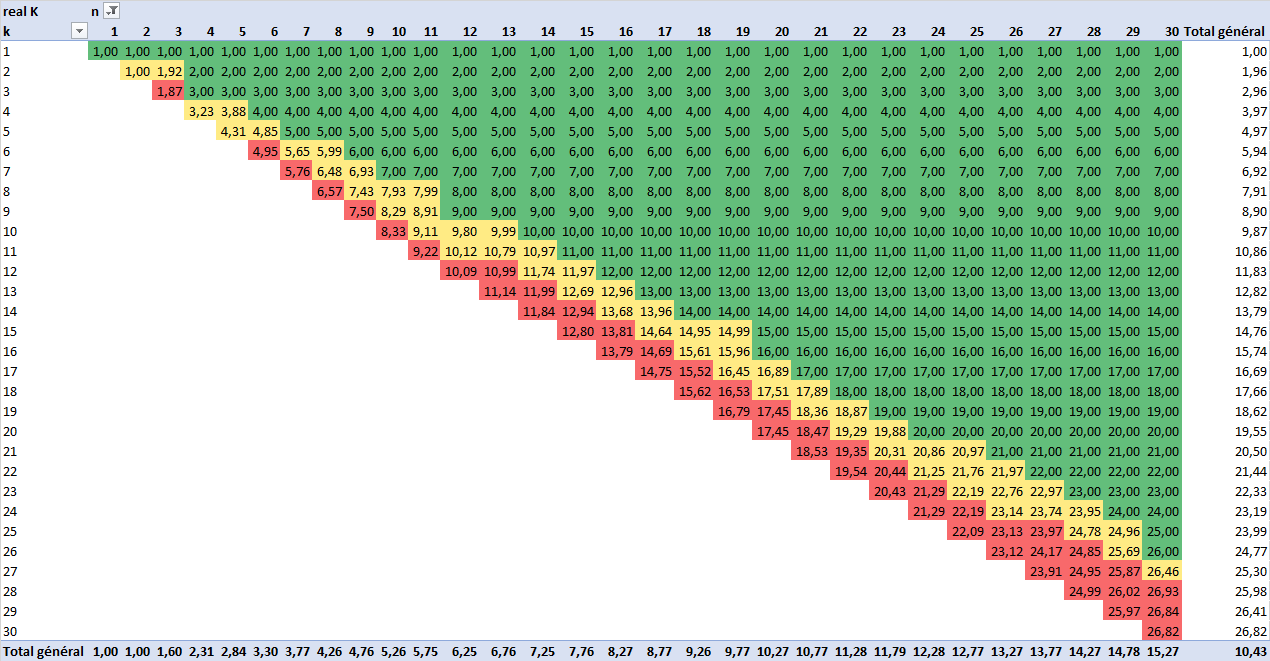
\includegraphics[width=\textwidth]{realK30.png} \end{center}

            On peut voir que l'algorithme, pour $N=30$, arrive à placer toutes les reines jusqu'à $K=N-4$, entre $K=N-4$ et $K=N-3$ il manque $1$ reine. Plus $K$ tend vers $N$, plus le placement d'une reine au hasard est difficile. Plus $N$ est grand, plus le problème apparait tôt.

			\begin{center} 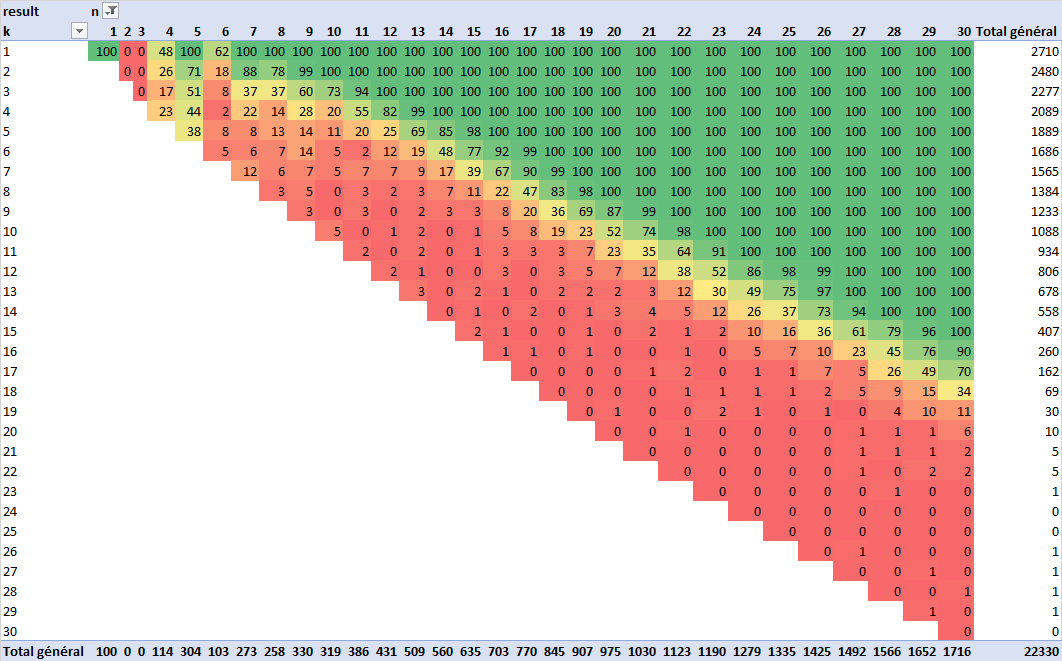
\includegraphics[width=\textwidth]{result30.png} \end{center}

            Le solveur arrive, pour $N=30$, à trouver des solutions pour $K<N/2$ et en trouve un certain nombre pour $2N/3<K<N/2$. Plus N est grand, plus le solveur arrouve à trouver des solutions pour un K grand.

			\begin{center} 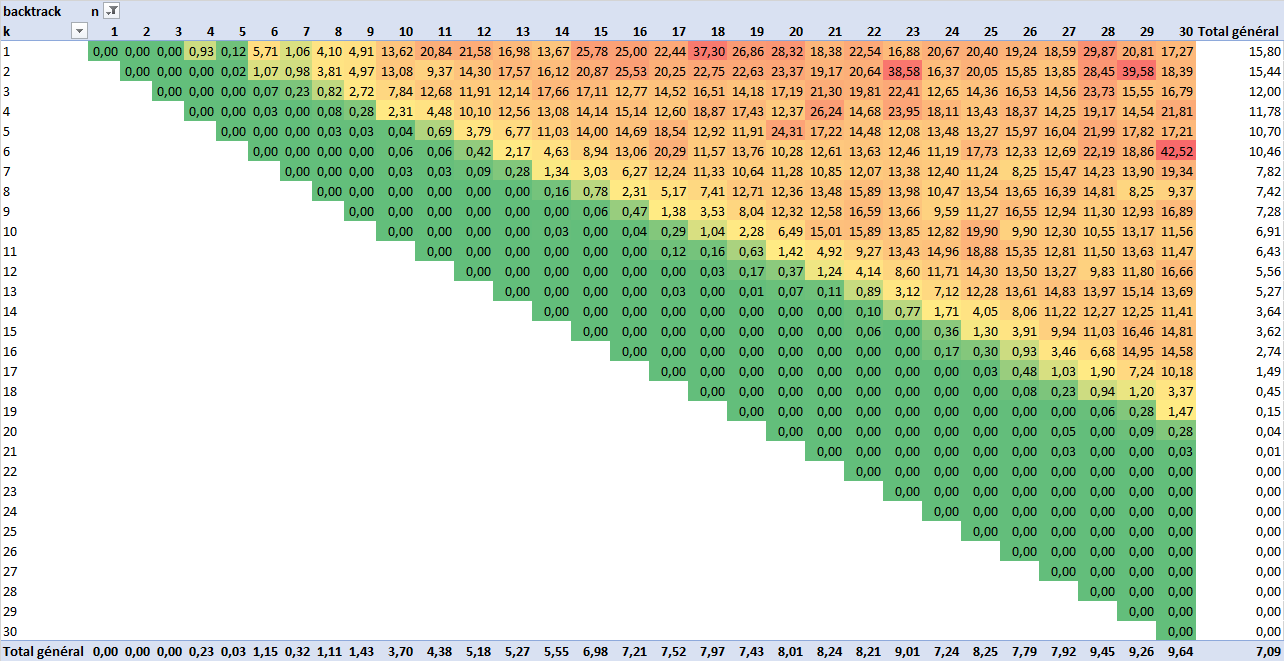
\includegraphics[width=\textwidth]{backtrack30.png} \end{center}

			Globalement, le nombre de backtrack est bien inférieur lorsque l'on place des points. Ce nombre trouve un minima vers $K=N/2$. Le solveur dit 0 lorsque celui-ci ne trouve pas de solution.

        \section{Sources}
            L'intégralité de mon code source et mes résultats allant jusqu'à $N=80$ (fichier de sortie et images) sont disponibles sur mon GitHub:
            \href{https://github.com/kevingrillet/KQueens}{https://git.io/vNtHi}
% Fin du document
\end{document}
